\documentclass[12pt, a4paper, oneside]{ctexart}
\usepackage{amsmath, amsthm, amssymb, bm, color, graphicx, geometry, mathrsfs,extarrows, braket, booktabs, array, xcolor, fontspec, appendix, float, subfigure, wrapfig}
\usepackage[colorlinks,linkcolor=red,anchorcolor=blue,citecolor=blue,urlcolor=blue,menucolor=black]{hyperref}

%%%% 设置英文字体 %%%%
\setmainfont{Times New Roman}
\setsansfont{Calibri}
\setmonofont{Consolas}

%%%% 设置代码块 %%%%
% 在vscode中使用minted需要先配置python解释器, Ctrl+Shift+P, 输入Python: Select Interpreter选择安装了Pygments的Python版本. 再在setting.json中xelatex和pdflatex的参数中加入 "--shell-escape", 即可
% TeXworks中配置方法参考: https://blog.csdn.net/RobertChenGuangzhi/article/details/108140093
\usepackage{minted}
\renewcommand{\theFancyVerbLine}{
    \sffamily\textcolor[rgb]{0.5,0.5,0.5}{\scriptsize\arabic{FancyVerbLine}}} % 修改代码前序号大小
\newmintinline{python}{linenos, breaklines, frame=lines, python3}  % 使用\pythoninline{代码}
\newminted{python}{linenos, breaklines, frame=lines, python3}  % 使用\begin{pythoncode}代码\end{pythoncode}
\newmintedfile{python}{linenos, breaklines, frame=lines, python3}  % 使用\pythonfile{代码地址}

%%%% 设置字号 %%%%
\newcommand{\chuhao}{\fontsize{42pt}{\baselineskip}\selectfont}     % 初号
\newcommand{\xiaochuhao}{\fontsize{36pt}{\baselineskip}\selectfont} % 小初号
\newcommand{\yihao}{\fontsize{28pt}{\baselineskip}\selectfont}      % 一号
\newcommand{\erhao}{\fontsize{21pt}{\baselineskip}\selectfont}      % 二号
\newcommand{\xiaoerhao}{\fontsize{18pt}{\baselineskip}\selectfont}  % 小二号
\newcommand{\sanhao}{\fontsize{15.75pt}{\baselineskip}\selectfont}  % 三号
\newcommand{\sihao}{\fontsize{14pt}{\baselineskip}\selectfont}      % 四号
\newcommand{\xiaosihao}{\fontsize{12pt}{\baselineskip}\selectfont}  % 小四号
\newcommand{\wuhao}{\fontsize{10.5pt}{\baselineskip}\selectfont}    % 五号
\newcommand{\xiaowuhao}{\fontsize{9pt}{\baselineskip}\selectfont}   % 小五号
\newcommand{\liuhao}{\fontsize{7.875pt}{\baselineskip}\selectfont}  % 六号
\newcommand{\qihao}{\fontsize{5.25pt}{\baselineskip}\selectfont}    % 七号

%%%% 设置行间距与页边距 %%%%
\linespread{1.4}
\geometry{left=2.5cm, right=2.5cm, top=2.5cm, bottom=2.5cm}

%%%% 定理类环境的定义 %%%%
\newtheorem{example}{例}            % 整体编号
\newtheorem{theorem}{定理}[section] % 定理按section编号
\newtheorem{definition}{定义}
\newtheorem{axiom}{公理}
\newtheorem{property}{性质}
\newtheorem{proposition}{命题}
\newtheorem{lemma}{引理}
\newtheorem{corollary}{推论}
\newtheorem{remark}{注解}
\newtheorem{condition}{条件}
\newtheorem{conclusion}{结论}
\newtheorem{assumption}{假设}
\numberwithin{equation}{section}  % 公式按section编号 (公式右端的小括号)
\newtheorem{algorithm}{算法}

%%%% 图片相对路径 %%%%
\graphicspath{{figure/}} % 当前目录下的figure文件夹, {../figure/}则是父目录的figure文件夹

\everymath{\displaystyle} % 默认全部行间公式, 想要变回行内公式使用\textstyle
\DeclareMathOperator*\uplim{\overline{lim}}     % 定义上极限 \uplim_{}
\DeclareMathOperator*\lowlim{\underline{lim}}   % 定义下极限 \lowlim_{}
\let\leq=\leqslant % 简写小于等于\leq (将全部leq变为leqslant)
\let\geq=\geqslant % 简写大于等于\geq (将全部geq变为geqslant)

%%%% 一些宏定义 %%%%%
\def\bd{\boldsymbol}        % 加粗(向量) boldsymbol
\def\disp{\displaystyle}    % 使用行间公式 displaystyle(默认)
\def\tsty{\textstyle}       % 使用行内公式 textstyle
\def\sign{\text{sign}}      % sign function
\def\wtd{\widetilde}        % 宽波浪线 widetilde
\def\R{\mathbb{R}}          % Real number
\def\C{\mathbb{C}}          % Complex number
\def\N{\mathbb{N}}     
\def\d{\mathrm{d}}          % differential operator
\def\e{\mathrm{e}}          % Euler's number
\def\i{\mathrm{i}}          % imaginary number
\def\re{\mathrm{Re}}        % Real part
\def\im{\mathrm{Im}}        % Imaginary part
\def\L{\mathcal{L}}         % Loss function
\def\wdh{\widehat}          % 宽帽子 widehat
\def\ol{\overline}          % 上横线 overline
\def\ul{\underline}         % 下横线 underline
\def\add{\vspace{1ex}}      % 增加行间距
\def\del{\vspace{-3.5ex}}   % 减少行间距

%%%% 正文开始 %%%%
\begin{document}

%%%% 以下部分是正文 %%%%  
\section*{非负可测函数的Lebesgue积分的等价性\\
{\xiaosihao 吴天阳\ 强基数学002\quad 学号: 2204210460}
}


\begin{definition}
    设$E$是$\R^q$中的可测集, $f(x)$是$E$上的非负可测函数.

    $(1)$ 若$E$为有界集, 对$[0,\infty)$上任一分割
    \begin{equation*}
        H:0=y_0<y_1<\cdots<y_i<\cdots,\quad (y_i\to\infty),
    \end{equation*}
    记$\lambda(H) = \sup_i(y_i-y_{i-1})$, $E_i = E[y_{i-1}\leq f<y_i]$. $\ol{\sigma}(H,f) = \sum_{i=1}^\infty y_im(E_i)$, $\ul{\sigma}(H, f) = \sum_{i=1}^\infty y_{i-1}m(E_i)$. 任取分割列
    \begin{equation*}
        H_1\leq H_2\leq \cdots\leq H_n\leq \cdots,\quad(\lambda(H_n)\to 0),
    \end{equation*}
    其中$H_{n-1}\leq H_n$表示$H_n$为$H_{n-1}$的加细.\add

    定义Lebesgue积分$\int_Ef(x)\,\d x$为当$\lambda(H_n)\to 0$时, $\ol{\sigma}(H_n,f)$与$\ul{\sigma}(H_n,f)$的共同极限$a\ (0\leq a\leq \infty)$.

    $(2)$ 若$E$为无界集, 则定义Lebesgue积分为$\int_Ef(x)\,\d x = \lim_{n\to\infty}\int_{E_n}f(x)\,\d x$, 其中$E_n$与定义$1(2)$相同.
\end{definition}
\begin{definition}
    设$E$为$\R^q$中的可测集.

    $(1)$设$\varphi(x)=\sum_{i=1}^nc_i\chi_{E_i}(x)$为$E$上的非负简单函数, 其中$E = \bigcup_{i=1}^nE_i$, 各$E_i$为互不相交的可测集, $\chi_{E_i}(x)$为$E_i$的特征函数, 则定义Lebesgue积分为$\int_{E}\varphi(x)\,\d x=\sum_{i=1}^nc_im(E_i)$.

    $(2)$设$f(x)$为$E$上的非负可测函数, 则定义Lebesgue积分为
    \begin{equation*}
        \int_Ef(x)\,\d x=\sup\left\{\int_E\varphi(x)\,\d x:\varphi\text{为}E\text{上的简单函数, 且}0\leq \varphi\leq f\right\}.
    \end{equation*}
\end{definition}
上述定义中, 当$\int_Ef(x)\,\d x < \infty$时, 称$f(x)$在$E$上Lebesgue可积.

\begin{lemma}
    设$\{E_n\}$为$\R^q$中递增的可测集列, 且$E=\bigcup_{n=1}^\infty E_n$, $\varphi(x)$为$E$上非负简单函数, 则在定义$2(1)$意义下, 有$\int_E\varphi(x)\,\d x =\lim_{n\to\infty}\int_{E_n}\varphi(x)\,\d x$.
\end{lemma}
\begin{proof}(参考\cite{zmq})
    由于$\{|\varphi(x)|\chi_{E_k}(x)\}$是非负渐升列, 且有
    \begin{equation*}
        \lim_{k\to\infty}|\varphi(x)|\chi_{E_k}(x)=|\varphi(x)|,\quad (x\in E),
    \end{equation*}
    由Beppo Levi非负渐升列积分定理可知
    \begin{align*}
        \int_E|\varphi(x)|\,\d x=\lim_{k\to\infty}\int_{E}|\varphi(x)|\chi_{E_k}(x)\,\d x = \lim_{k\to\infty}\int_{E_k}|\varphi(x)|\,\d x < \infty,
    \end{align*}
    即$\varphi\in L(E)$. 又由于在$E$上有$(k=1,2,\cdots)$, 则
    \begin{equation*}
        \lim_{k\to\infty}\varphi(x)\chi_{E_k}(x)=\varphi(x),\quad |\varphi(x)\chi_{E_k}(x)|\leq |\varphi(x)|,
    \end{equation*}
    故根据控制收敛定理可得
    \begin{equation*}
        \int_E\varphi(x)\,\d x=\lim_{k\to\infty}\varphi(x)\,\d x.
    \end{equation*}
\end{proof}
\begin{lemma}
    设$E$为$\R^q$中的可测集, $f(x)$是$E$上的非负可测函数.

    $(1)$ 对$E$上任意简单函数$\varphi(x):0\leq \varphi(x)\leq f(x)$, 恒有$\int_{E}\varphi(x)\,\d x\leq \int_{E}f(x)\,\d x$;\add

    $(2)$ $f(x)$在$E$上Lebesgue可积, 则任意的$\varepsilon > 0$, 存在$E$上的简单函数$\varphi(x):0\leq \varphi(x)\leq f(x)$, 使$\int_E\varphi(x)\,\d x>\int_Ef(x)\,\d x-\varepsilon$. 其中$\int_Ef(x)\,\d x$与定义$1$相同, $\int_E\varphi(x)\,\d x$与定义$2(1)$相同.
\end{lemma}
\begin{proof}
    当$E$为有界集时, 由定义$1(1)$与定义$2(1)$得证(见\cite{sbhs}). 以下证明$E$为无界的情形. 设$E$是$\R^q$中的可测集, $f(x)$是$E$上的非负可测函数, 记
    \begin{equation*}
        K_n=\{(x_1,x_2,\cdots, x_q)\}:|x_i|\leq n,\ i=1,2,\cdots, q\},\ E_n=E\cap K_n.
    \end{equation*}

    (1) 对任意的$n\in\N$, 在$E_n$上有$0\leq \varphi(x)\leq f(x)$, 而$E_n$有界, 且定理对有界集成立. 故
    \begin{equation*}
        \int_{E_n}\varphi(x)\,\d x\leq \int_{E_n}f(x)\,\d x.
    \end{equation*}
    又由于$\{E_n\}$递增, 且$E=\bigcup_{n=1}^\infty E_n$, 由引理$1$与定义$1(2)$的知, 当$n\to\infty$时
    \begin{equation*}
        \int_E\varphi(x)\,\d x\leq \int_{E}f(x)\,\d x.
    \end{equation*}

    (2) 记$a=\int_Ef(x)\,\d x < \infty$, 由定义$1(2)$知$a=\lim_{n\to\infty}\int_{E_n}f(x)\,\d x$, 故对任意的$\varphi > 0$, 取$N$使得$a\geq \int_{E_N}f(x)\,\d x>a-\frac{\varphi}{2}$. 由于$E_N$有界, 故存在$E_N$上的简单函数$\varphi_N(x):0\leq \varphi_N(x)\leq f(x)$, 使得\begin{equation*}
        \int_{E_N}\varphi_N(x)\,\d x > \int_{E_N}f(x)\,\d x-\frac{\varepsilon}{2}.
    \end{equation*}
    令
    \begin{equation*}
        \varphi(x) = \begin{cases}
            \varphi_N(x), &\quad x\in E_N,\\
            0,&\quad x\in E-E_N,
        \end{cases}
    \end{equation*}
    则$\varphi(x)$为$E$上简单函数, 且$0\leq \varphi(x)\leq f(x)$, 而
    \begin{equation*}
        \int_{E}\varphi(x)\,\d x=\int_{E_N}\varphi_N(x)\,\d x > \int_{E_N}f(x)\,\d x-\frac{\varepsilon}{2}>a-\varepsilon.
    \end{equation*}
\end{proof}
设$E$为$\R^q$中测度有限的可测集, $f(x)$是$E$上的有界可测函数, 且$f(E)\subset (\alpha, \beta)$, 对$[\alpha, \beta]$上任一分隔
\begin{equation*}
    D:\alpha = y_0 < y_1<\cdots < y_n=\beta.
\end{equation*}
令$\lambda(D) = \max_i(y_i-y_{i-1})$, $E_i = E(y_{i-1}\leq f < y_i)$, 引入Lebesgue大和$S$和小和$s$
\begin{equation*}
    S(D, f) = \sum_{i=1}^ny_im(E_i),\quad s(D, f) = \sum_{i=1}^ny_{i-1}m(E_i).
\end{equation*}
记集类$\mathcal{D} := \{D:\lambda(D) < \infty\}$, 对于$D_1, D_2\in \mathcal{D}$, 若$D_1\subset D_2$, 则称$D_2$为$D_1$的加细, 记为$D_1\leq D_2$, 此时有$\lambda(D_2)\leq \lambda(D_1)$. 于是有如下性质
\begin{lemma}
    设有分划列$D_1\leq D_2\leq \cdots \leq D_n\leq \cdots$, $\lambda(D_n)\to 0$. 则$s(D_n),S(D_n)$趋于同一极限$a$, $a$为有限数或$\infty$.
\end{lemma}
\begin{proof}
    由于$S(D_n) - s(D_n)\leq \sum_{n}(y_{n+1}-y_n)m(E_n)\leq \lambda(D_n)m(E)$, 而$m(E) < \infty$, 所以当$\lambda(D_n)\to 0$时, $S(D_n)-s(D_n)\to 0$.

    若$S(D_1)=\infty$, 则$S(D_1)=\infty$, 从而一切$s(D_n)$与$S(D_n)$均为$\infty$, 此时$a=\infty$. 事实上, 若设$S(D_1) < \infty$, 则由于$S(D_1)-s(D_1)\leq \lambda(D_1)m(E) < \infty$, 故当$s(D_1) < \infty$时, 必有$S(D_1) < \infty$, 这与$S(D_1)=\infty$矛盾.

    若$S(D_1) < \infty$, 则
    \begin{equation*}
        s(D_1)\leq s(D_2)\leq \cdots \leq s(D_n)\leq \cdots \leq S(D_1) < \infty
    \end{equation*}
    可见, 此时$\{s(D_n)\}$为单调上升有界数列, 故必然有有限极限, 记为$a$, 同理$\{S(D_n)\}$为单调下降有界数列, 必有极限, 记为$c$. 易得$a=c$, 否则, 若$a<c$, 则
    \begin{equation*}
        S(D_n)-s(D_n)\geq c-a >0
    \end{equation*}
    这与$S(D_n)-s(D_n)\to 0$矛盾.
\end{proof}
\begin{lemma}
    若引理$3$中$a=\infty$, 则任意的$M>0$, 存在简单函数$\varphi:0\leq \varphi\leq f$, 且使
    \begin{equation*}
        \int_E\varphi(x)\,\d m\geq M
    \end{equation*}
    成立.
\end{lemma}
\begin{proof}
    根据引理$3$证明, 存在分划\begin{equation*}
        D:0\leq y_0 < y_1 < \cdots < y_n < \cdots,
    \end{equation*}
    使得$s(D) = \infty$, 即$s(D) = \sum_{n=0}^\infty y_nm(E_n)=\infty$. 因此可取充分大的$N$使得
    \begin{equation*}
        \sum_{n\leq N}y_nm(E_n)>M.
    \end{equation*}
    定义简单函数$\varphi$为
    \begin{equation*}
        \varphi(x)=\begin{cases}
            y_n,&\quad x\in E_n,n\leq N,\\
            0,&\quad\mathtt{otherwise}.
        \end{cases}
    \end{equation*}
    则$0\leq \varphi\leq f$且$\int_E\varphi(x)\,\d m = \sum_{n\leq N}y_nm(E_n)>M$.
\end{proof}
\begin{lemma}
    对于简单函数$\varphi:0\leq \varphi \leq f$, 恒有$\int_E\varphi(x)\,\d m\leq a$, 其中$a$为引理$3$中所述.
\end{lemma}
\begin{proof}
    由引理$3$证明, 任意的$\varphi>0$, 存在$D\in \mathcal{D}$, 使得$S(D) < a+\varepsilon$.

    设$S(D) = \sum_{n=0}^\infty y_{n+1}m(E_n)$, 由于简单函数$\varphi$只取有限个值, 于是有$N$, 使得$\varphi\leq y_{N+1}$.

    若定义另一简单函数$\psi$为
    \begin{equation*}
        \psi(x)=\begin{cases}
            y_{n+1},&\quad x\in E_n(n\leq N),\\
            y_{N+1},&\quad \mathtt{otherwise}.
        \end{cases}
    \end{equation*}
    那么有
    \begin{equation*}
        \int_E\varphi(x)\,\d m\leq \int_{E}\psi(x)\,\d m.
    \end{equation*}
    而
    \begin{equation*}
        \int_E\psi(x)\,\d m=\sum_{n\leq N}y_{n+1}m(E_n)+y_{N+1}m(E-\bigcup_{n\leq N}E_n)\leq S(D) <a+\varepsilon.
    \end{equation*}
    则$\int_{E}\varphi(x)\,\d m < a+\varepsilon$.

    由$\varepsilon$的任意性可知, $\int_E\varphi(x)\,\d m\leq a$.
\end{proof}
\begin{lemma}
    若上述极限$a<\infty$, 则任意的$\varepsilon >0$, 存在简单函数$\varphi:0\leq \varphi\leq f$, 使得$\int_{E}\varphi(x)\,\d m > a-\varepsilon$.
\end{lemma}
\begin{proof}
    由引理$3$证明, 必存在分划$D$, 使得$s(D) > a-\frac{\varepsilon}{2}$. 设$s(D) = \sum_{n}y_nm(E_n)$, 有可取充分大的$N$, 使得$\sum_{n > N}y_nm(E_n) < \frac{\varepsilon}{2}$, 则$\sum_{n \leq N}y_nm(E_n)>a-\varepsilon$.

    定义简单函数$\varphi$为
    \begin{equation*}
        \varphi(x)= \begin{cases}
            y_n,&\quad x\in E_n(n\leq N),\\
            0,&\quad \mathtt{otherwise}.
        \end{cases}
    \end{equation*}
    那么有$0\leq \varphi\leq f$, 且$\int_E\varphi(x)\,\d m=\sum_{n\leq N}y_nm(E_n) > a-\varepsilon$.
\end{proof}

\paragraph*{Lebesgue积分的等价性证明}
\begin{proof}
    设$\int_Ef(x)\,\d x$在定义$1$与定义$2$下的值分别为$b$和$c$, 即
    \begin{align*}
        b =&\ \lim_{n\to\infty}\int_{E_n}f(x)\,\d x,\\
        c =&\ \sup\left\{\int_E\varphi(x)\,\d x:\varphi(x)\text{为}E\text{上简单函数, 且}0\leq \varphi(x)\leq f(x)\right\},
    \end{align*}
    其中$E_n=E\cap K_n$的定义与引理$2$中一致, 则两个定义等价只需证明$b=c$, 以下分为两种情况:

    $(1)$ 当$E$为有界集时,(证明参考\cite{sbhs})
    
    $(i)$ 若$m(E(f=\infty))>0$, 则$b=\infty$, 另一方面, 若记$\delta = m(E(f=\infty))$, 则对任何一正数$M>0$, 可定义一简单函数为:
    \begin{equation*}
        \varphi(x)=\begin{cases}
            \frac{M}{\delta},&\quad x\in E(f=\infty),\\
            0,&\quad x\in E-E(f=\infty).
        \end{cases}
    \end{equation*}
    于是对于此$\varphi$有$0\leq \varphi\leq f$, 而且$\int_{E}\varphi(x)\,\d m = M$. 这说明$c=\infty$, 所以$b=c$成立.\add

    $(ii)$ 若$f$是几乎处处有限时, 此时$b$有两种可能.
    
    当$b=\infty$时, 由引理$4$可得$c=b=\infty$;
    
    当$b<\infty$时, 由引理$5$可知, 任意的$\varepsilon > 0$, $c < b+\varepsilon$, 又由引理$6$可知$c>b-\varepsilon$. 所以$|b-c| < \varepsilon$, 因此由$\varepsilon$的任意性可知$b=c$.

    $(2)$ 当$E$为无界集时,(证明参考\cite{djx})
    
    $(i)$ $b=\infty$, 则任意的$M>0$, 存在$N\in \N$, 使得在定义$1$下$\int_{E_N}f(x)\,\d x>M$, 因为$E_N = E\cap K_n$有界, 故由$(1)$可知$\int_{E_N}f(x)\,\d x$在两个定义下相等, 于是存在$E_N$上的简单函数$\varphi_N(x):0\leq \varphi_N(x)\leq f(x)$使得$\int_{E_N}\varphi_N(x)\,\d x > M$.

    令
    \begin{equation*}
        \varphi(x) = \begin{cases}
            \varphi_N(x), &\quad x\in E_N,\\
            0,&\quad x\in E-E_N,
        \end{cases}
    \end{equation*}
    则$\varphi(x)$为$E$上的简单函数, $0\leq \varphi(x)\leq f(x)$, 且$\int_E\varphi(x)\,\d x=\int_{E_N}\varphi_N(x)\,\d x > M$. 于是$c>M$, 所以$c=\infty$.

    $(ii)$ $b < \infty$, 由引理$2(1)$可知 $c\leq b$, 又由引理$2(2)$可知, 任意的$\varepsilon > 0$, 存在$E$上简单函数$\varphi(x):0\leq \varphi(x)\leq f(x)$, 使得$\int_E\varphi(x)\,\d x > b-\varepsilon$, 于是$c>b-\varepsilon$, 从而$c\geq b$, 所以$b=c$.

\end{proof}

\begin{thebibliography}{99}
    \bibitem{sbhs} 王戍堂, 温作吉. 实变函数论[M]. 西安:西北大学出版社, 2001.
    \bibitem{zmq} 周民强. 实变函数论[M]. 北京:北京大学出版社, 1985.
    \bibitem{djx} 张永峰. 非负可测函数L积分的定义及其等价性[J]. 纺织高校基础科学学报, 2007.9.
\end{thebibliography}

\end{document}

\iffalse
%%%% 表格模板 %%%%
\renewcommand\arraystretch{0.8} % 设置表格高度为原来的0.8倍
\begin{table}[!htbp] % table标准
    \centering % 表格居中
    \begin{tabular}{p{1cm}<{\centering}p{1cm}<{\centering}p{3cm}<{\centering}p{5cm}<{\centering}} % 设置表格宽度
    %\begin{tabular}{cccc}
        \toprule
        $x_i$ & $f[x_1]$ & $f[x_i, x_{i+1}]$ & $f[x_i, x_{i+1}, x_{i+2}]$ \\
        \midrule
        $x_0$ & $f(x_0)$ &                  &                          \\
        $x_0$ & $f(x_0)$ & $f'(x_0)$        &                          \\
        $x_0$ & $f(x_1)$ & $\frac{f(x_1)-f(x_0)}{x_1-x_0}$ & $\frac{f(x_1)-f(x_0)}{(x_1-x_0)^2}-\frac{f'(x_0)}{x_1-x_0}$\\
        \bottomrule
    \end{tabular}
\end{table}

%%%% 文字环绕图片, 标题加注释 %%%%
{ % 一般将文字环绕部分的图和文字, 用大括号括起来, 避免对文字外的格式发生影响
\begin{wrapfigure}[13]{r}{.5\linewidth} % 文字环绕行数为13行, 图片靠右 (l为靠左), 图片占0.5的行宽
    \centering
    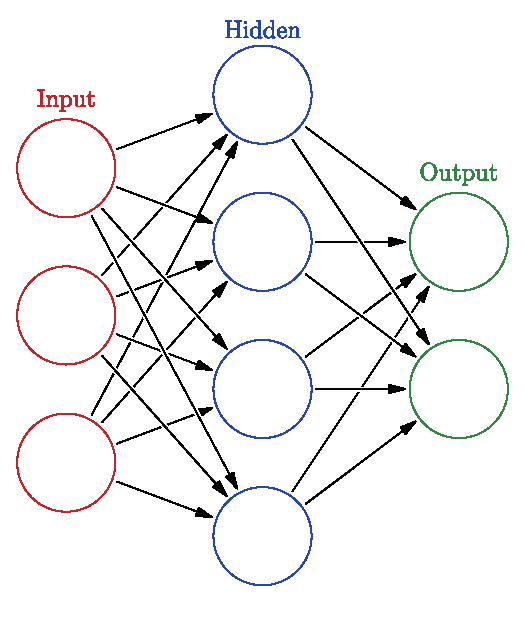
\includegraphics[scale=0.7]{neural_network.eps} % scale=0.7按比例缩放70%
    \caption{神经网络结构\protect\footnotemark[1]} % 记得加\protect, 设置1号脚标
    \label{figure-神经网络结构}
\end{wrapfigure}
\footnotetext[1]{图片来源: \url{https://en.wikipedia.org/wiki/File:Colored_neural_network.svg}}
文字文字
}

%%%% 普通图片, 标题加注释 %%%%
\begin{figure}[htbp] % h: 当前位置, t: 顶部, b: 底部, p: 浮动页, 这样组合指的是使用这个顺序进行排版
    \centering
    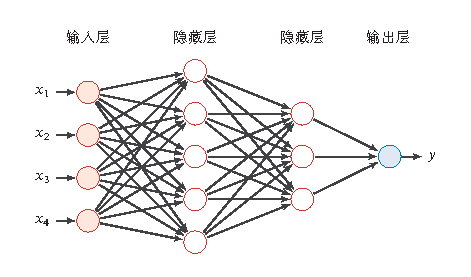
\includegraphics[scale=0.5]{前馈神经网络.eps}
    \caption{前馈神经网络\protect\footnotemark[1]}
    \label{figue-前馈神经网络}
\end{figure}
\footnotetext[1]{图片来源: 邱锡鹏, 神经网络与深度学习 \cite{ref-qxp}, 第92页}

%%%% 多组图 %%%%
    \begin{figure}[htbp]
        \centering
        \subfigure[迭代1次]  % 子图的标题
        {
            % 如果一行放三个图改成0.3\linewidth即可
            \begin{minipage}[b]{.45\linewidth}  % 0.45排版行距, 即一行放2个图, 一行放不下就换行
                \centering
                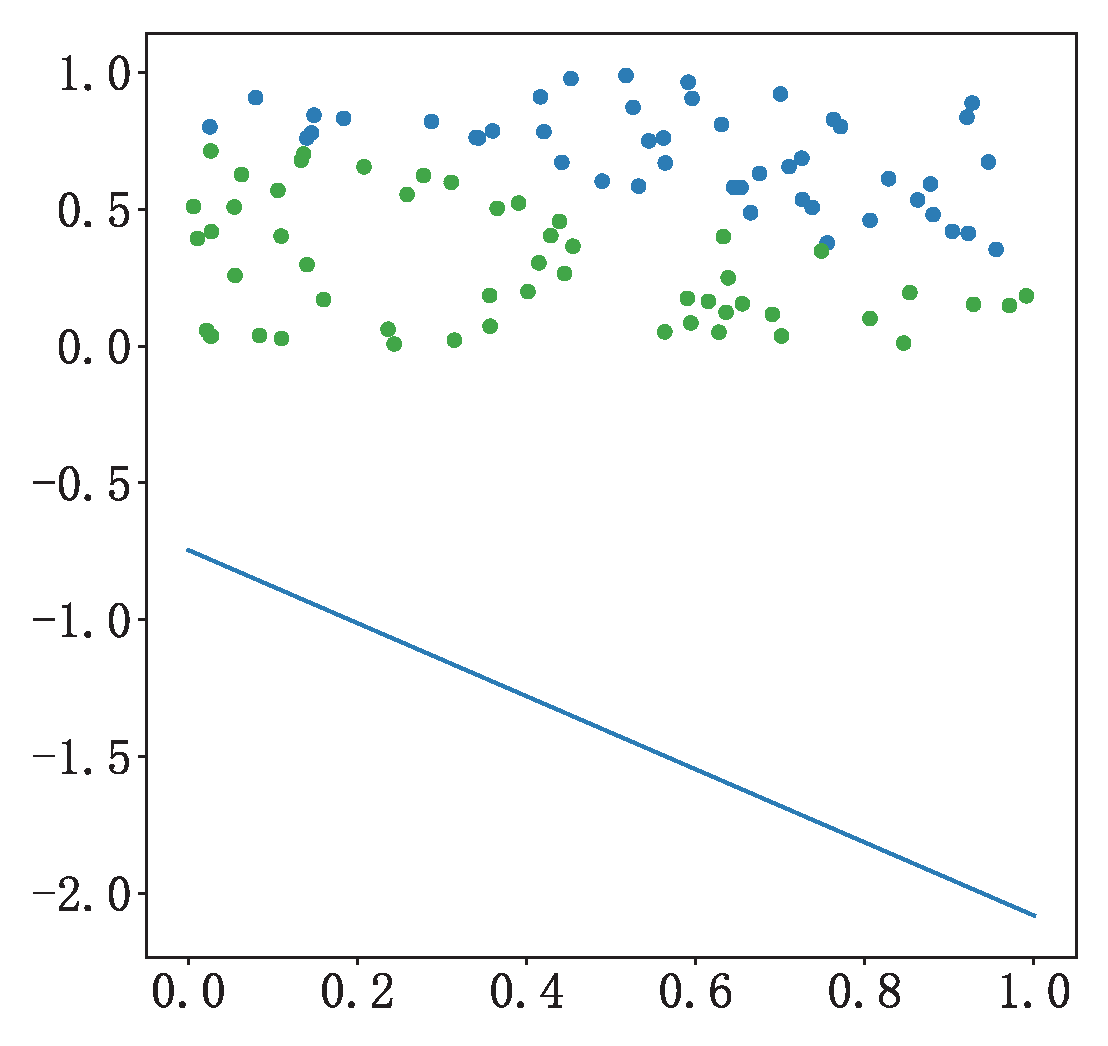
\includegraphics[scale=0.35]{1.eps}
            \end{minipage}
        }
        \subfigure[迭代100次]
        {
            \begin{minipage}[b]{.45\linewidth}
                \centering
                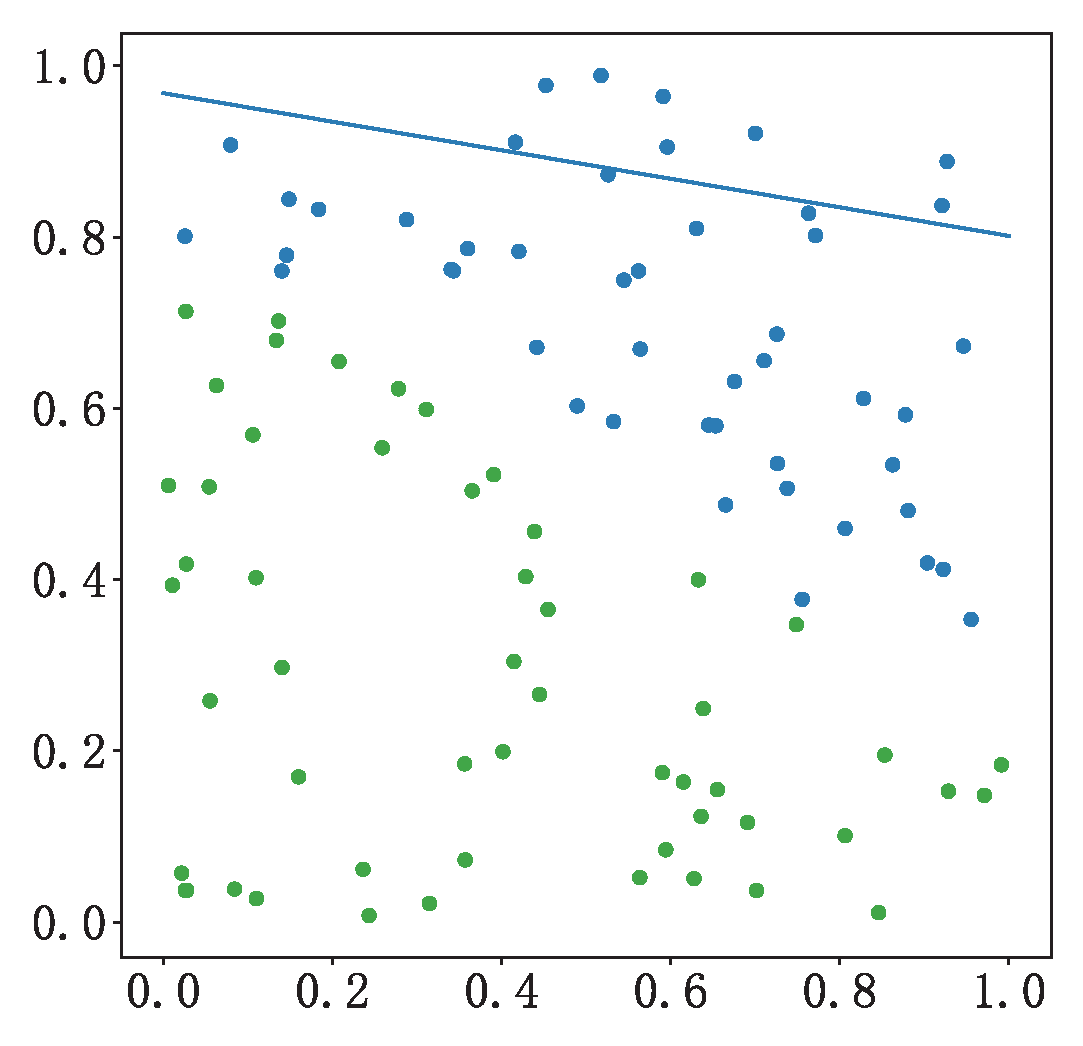
\includegraphics[scale=0.35]{100.eps}
            \end{minipage}
        }
        \subfigure[迭代500次]
        {
            \begin{minipage}[b]{.45\linewidth}
                \centering
                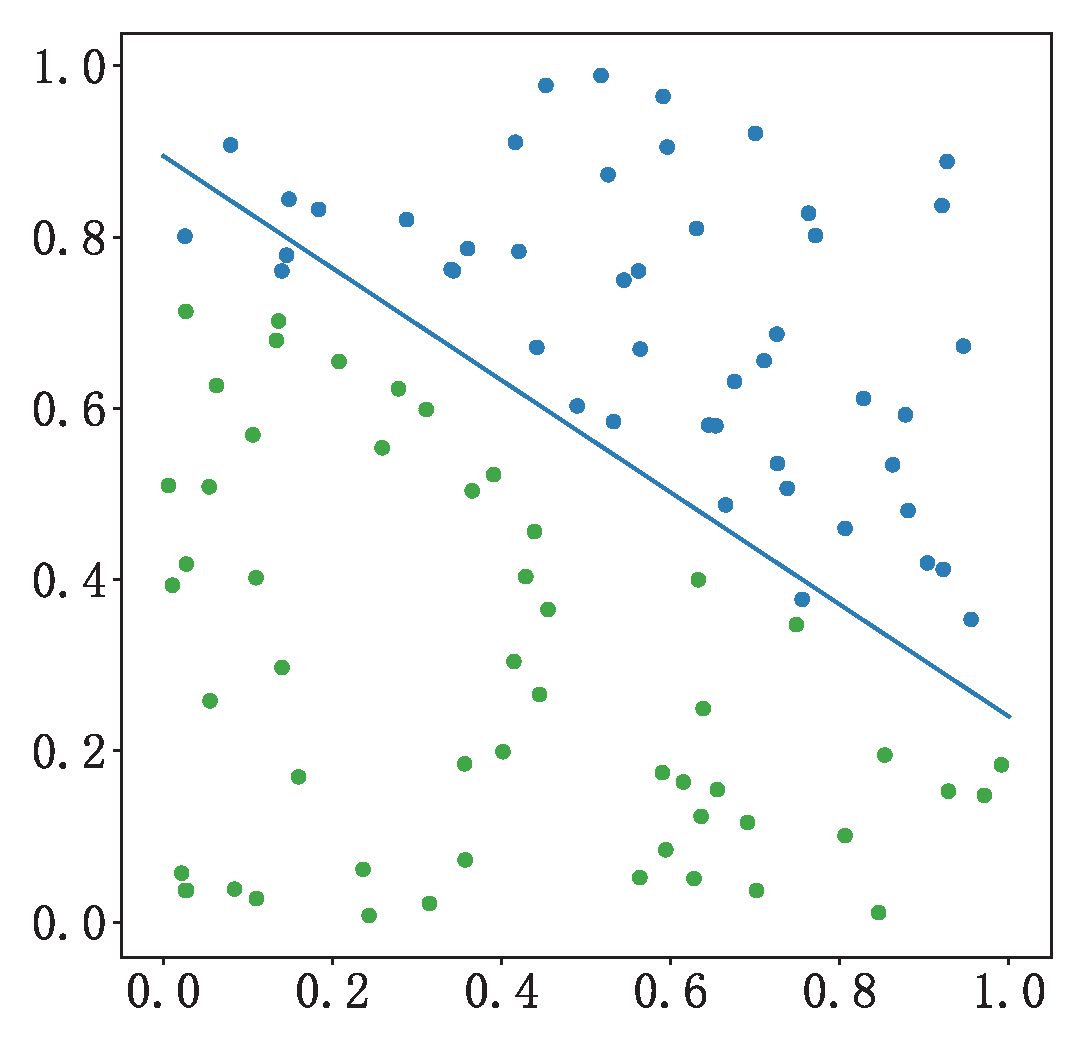
\includegraphics[scale=0.35]{500.eps}
            \end{minipage}
        }
        \subfigure[迭代2000次]
        {
            \begin{minipage}[b]{.45\linewidth}
                \centering
                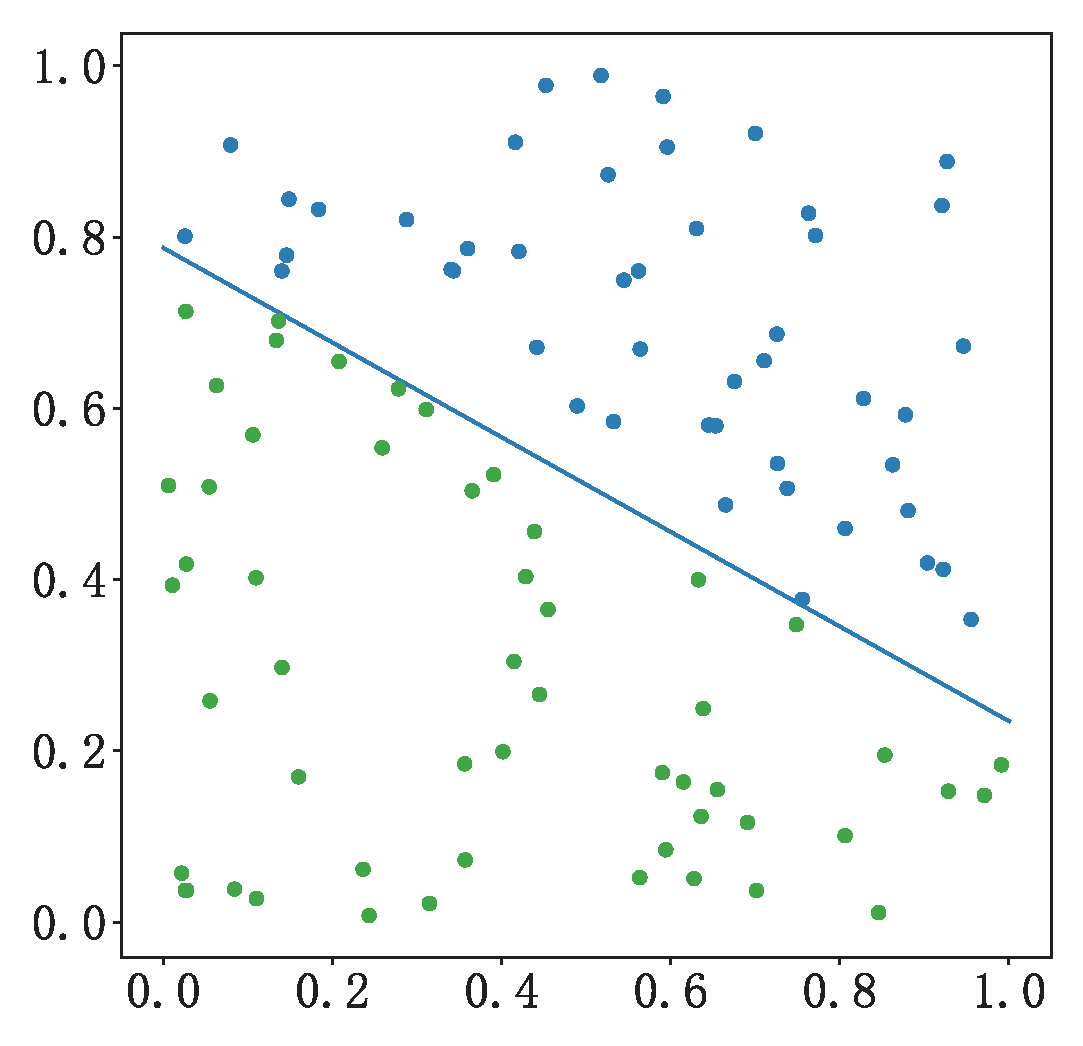
\includegraphics[scale=0.35]{2000.eps}
            \end{minipage}
        }
        \caption{迭代过程图}
        \label{figure-迭代过程图}
    \end{figure}
\fi
